\section{微分形式在流形上的积分}

\noindent\textbf{1. 微分形式在 $\mathbb R^n$ 上的积分}\quad
本节中我们将讨论一个微分流形 $M$ 上的微分形式 $\omega\in F^n(M)$（$\omega$ 的阶数与 $M$ 的维数相同）在 $M$ 上的积分问题。因为 $M$ 是光滑的，$F^n(M)$ 中的元素为 $\Lambda^n(M)$ 的 $C^\infty$ 切口，因此也是光滑的。在光滑的积分区域上对光滑的被积表达式作积分，黎曼积分就已经够用了。所以本章中的积分都限于黎曼积分而不去讨论第四章中的勒贝格积分，也就不必讨论 $M$ 上如何定义测度的问题。当然这不等于说在研究有关于流形的几何问题时用不着勒贝格积分。退一步说，至少要有黎曼度量才行。一个微分流形，如我们所已假设的，是豪斯多夫空间，而且满足第二可数性公理，在这个条件下，这个流形上一定有黎曼度量存在（证明见定理6），也可以证明它由此就是一个度量空间（证明略去），但是我们现在还没有利用这些结果。在这种情况下如何定义 $M$ 上的积分？办法就是利用 $M$ 上的局部坐标，把积分区域映射到 $\mathbb R^n$ 上去。这个映射尽管“我们说它是可微的”，却不涉及测度问题。设 $U\subset M$ 是一个坐标邻域，$\varphi:U\to\mathbb R^n$ 是坐标映射，记 $\varphi(U)=V$，$\omega$ 在 $\varphi$ 下之像为 $\Omega$，则
\[
 \Omega=a(x)\,dx^1\wedge\cdots\wedge dx^n.
\]
可是 $\omega$ 是 $\Omega$ 在 $\varphi$ 下的拉回：$\omega=\varphi^*\Omega$，于是我们定义
\begin{equation}
 \int_U\omega=\int_U\varphi^*\Omega=\int_{\varphi(U)}\Omega
 =\int_V a(x)\,dx^1\cdots dx^n,
 \tag{1}
\end{equation}
这就完全绕过了测度问题。

但是若在 $U$ 中有了另一个局部坐标 $(\psi,O),(y^1,\ldots,y^n)$，不失一般性，不妨设 $y$ 与 $x$ 坐标有相同定向。如果在新坐标系中 $\omega$ 成为
\[
 \widetilde\Omega=b(y)\,dy^1\wedge\cdots\wedge dy^n,
\]
则按(1)式，$\int_U\omega$ 应定义为
\begin{equation}
 \int_U\omega=\int_O\psi^*\widetilde\Omega
 =\int_{\psi(U)}\widetilde\Omega
 =\int b(y)\,dy^1\cdots dy^n.
 \tag{2}
\end{equation}
但由外微分形式的性质
\[
 b(y)dy^1\wedge\cdots\wedge dy^n
 =b(y(x))\frac{\partial(y^1,\ldots,y^n)}{\partial(x^1,\ldots,x^n)}
 dx^1\wedge\cdots\wedge dx^n
 =a(x)dx^1\wedge\cdots\wedge dx^n.
\]
即有
\[
 a(x)=b(y(x))J,
 \qquad
 J=\frac{\partial(y^1,\ldots,y^n)}{\partial(x^1,\ldots,x^n)}>0,
\]
因为 $y$ 与 $x$ 有相同定向，所以 $J=|J|$，而由黎曼积分中重积分之变量变换公式
\[
 \int a(x)dx^1\cdots dx^n
 =\int b(y(x))|J|dx^1\cdots dx^n
 =\int b(y)dy^1\cdots dy^n.
\]
因此这个定义是与坐标选择无关的，因而是合理的。研究微分流形上的积分理论时一个关键之点是要使所得的结果与坐标的选择无关，微分形式的性质正好保证了这一点。

尽管我们给出了(1)或(2)作为 $\omega$ 在 $U\subset M$ 上积分的定义的基础，其中仍有值得推敲的地方。因为例如对于(1)式，要使 $\int_Va(x)dx^1\cdots dx^n$ 有意义，应该要求 $\partial V$ 是勒贝格零测度集（第四章 §1），而且对 $a(x)$ 之光滑性不能只限于要求它在开集 $V$ 中光滑，因为这时 $a(x)$ 在 $\partial V$ 上仍可能很不规则，使得 $a(x)$ 在 $\overline V$ 上不一定可积（即所谓反常积分）。再说，在许多问题中 $\partial V$ 不一定是光滑的，例如它可以有边、有角等等，而处理这类问题总是很麻烦的。因此，我们干脆回到 $\mathbb R^n$，在其上重新建立起微分形式的积分理论，然后再来讨论如何把这些结果搬到微分流形上来。

在讲黎曼积分时我们常将积分区域分割成小的 $n$ 维长方体（以下为简单起见，就称它们为矩形，正如在第四章中称它们为区间一样）。现在我们要采取一种更有系统的分割方法，即分割一个空间为“单形”(simplex)，这不但是为了使读者有机会和拓扑学中的某些基本概念和方法早打交道，更是为了使读者注意到积分理论的组合学的侧面，这一点我们在第四章中已初步强调过了。

为了介绍什么是单形，先介绍一下线性空间 $V$ 中的仿射子空间 $A$，如果有 $V$ 的一个线性子空间 $W\subset V$，使
\[
 A=x_0+W,
\]
则称 $A$ 为 $V$ 之仿射子空间。从几何上看，仿射子空间无非是把一个线性子空间 $W$ 的原点移到 $x_0$ 点，这在几何上和物理上都是自然的。例如，以地球或以太阳为宇宙之中心均无不可。但仿射子空间在运算上显然有些麻烦：如果 $y_1,y_2\in A$，则 $y_1-y_2\in W$ 而不一定在 $A$ 中，$y_1+y_2$ 更不一定能写为 $x_0+(W\text{ 之某个元})$，除非 $x_0\in W$，而这时也就无所谓仿射空间 $A$ 了。今取 $W$ 的一个基底 $\{W_1,\ldots,W_k\}$，并令 $x_i=x_0+W_i$。当 $\{W_1,\ldots,W_k\}$ 线性无关时，由 $\sum_{i=1}^k\lambda_iW_i=0$，亦即由
\[
 \sum_{i=1}^k\lambda_i(x_i-x_0)=\sum_{i=0}^k\lambda_i x_i=0
\]
时可得 $\lambda_1=\cdots=\lambda_k=0$，这里 $\lambda_0=-(\lambda_1+\cdots+\lambda_k)$，从而 $\sum_{i=0}^k\lambda_i=0$。因此由 $\{W_1,\ldots,W_k\}$ 之线性无关，关于 $\{x_0,x_1,\ldots,x_k\}$ 可得到以下性质：若 $\sum_{i=0}^k\lambda_i x_i=0$ 以及 $\sum_{i=0}^k\lambda_i=0$ 可得 $\lambda_0=\cdots=\lambda_k=0$。这个性质我们说成是 $\{x_0,x_1,\ldots,x_k\}$ 仿射无关（即在仿射空间意义下无关）。反之由 $\{x_0,x_1,\ldots,x_k\}$ 仿射无关，必可得 $\{x_1-x_0,x_2-x_0,\ldots,x_k-x_0\}$ 线性无关。$\{x_0,x_1,\ldots,x_k\}$ 称为 $A$ 的一个仿射基底，因而仿射空间 $A$ 中的元一定可以表示为某个仿射基底的仿射组合如下：任取 $x\in A$，必有 $W$ 中一个元（它可以表示为 $\sum_{i=1}^k\mu_iW_i=\sum_{i=1}^k\mu_i(x_i-x_0)$），使
\begin{equation}
 x=x_0+\sum_{i=1}^k\mu_i(x_i-x_0)
 =\mu_0x_0+\sum_{i=1}^k\mu_i x_i
 =\sum_{i=0}^k\mu_i x_i,
 \qquad \mu_0=1-\sum_{i=1}^k\mu_i.
 \tag{3}
\end{equation}
形如(3)的表达式称为 $\{x_0,x_1,\ldots,x_k\}$ 的仿射组合，但
\begin{equation}
 \sum_{i=0}^k\mu_i=1\qquad (x_0,x_i\in V).
 \tag{4}
\end{equation}
最简单的例子是 $\{x_0,x_1\}$ 的仿射组合之集，即
\[
 L=\{\mu x_0+(1-\mu)x_1;\ \mu\in\mathbb R\}.
\]
它就是过 $x_0,x_1$ 两点的直线，它与 $V$ 的线性子空间不同，它不必经过原点。如果在 $L$ 中限制 $0\le\mu\le1$，则将得到 $L$ 上由 $x_0$ 到 $x_1$ 的线段（端点包括在内）。

有了仿射组合的概念以后，我们就可以定义单形了。

\noindent\textbf{定义1}\quad
$n$ 维线性空间 $V$ 中的 $k$ 维单形（这里 $0\le k\le n$），简称为 $k$ 单形($k$-simplex)，即 $k+1$ 个仿射无关的点 $\{x_0,x_1,\ldots,x_k\}$ 之如下的仿射组合的集合：
\begin{equation}
 \sigma_k=\langle x_0,x_1,\ldots,x_k\rangle
 =\left\{x;\ x=\sum_{i=0}^k\lambda_i x_i,
 0\le\lambda_i\le1,\ \sum_{i=0}^k\lambda_i=1\right\}.
 \tag{5}
\end{equation}
这些点称为 $\sigma_k$ 的顶点。

以上受了限制 $0\le\lambda_i\le1$ 的仿射组合是一个凸集，因此 $\sigma_k$ 就是由这些顶点所生成的闭凸集——或称凸包。$\lambda_i$ 称为 $x$ 点的第 $i$ 个重心坐标(barycentric coordinates)，我们常记之为 $b_i(x)=\lambda_i$。注意，$\sigma_k\subset V$ 乃是 $k$ 维空间的一个子集，所以其中的点的独立的坐标应有 $k$ 个分量，而现在有 $k+1$ 个 $\lambda_i$，所以它们并非本来意义的坐标，好在它们也不是独立的，因为有 $\sum_{i=0}^k\lambda_i=1$。

$0$ 单形就是一个点 $\{x_0\}$；$1$ 单形是一个线段；$2$ 单形是一个三角形。在考虑积分问题时必须考虑积分区域的定向，所以我们要规定单形(5)的定向。仿照 $\mathbb R^n$ 中定向即坐标按一定次序的排列，现在 $\sigma_k$ 的定向也就是把顶点 $\{x_0,x_1,\ldots,x_k\}$ 按一定次序的排列。以下 $\langle x_0,x_1,\ldots,x_k\rangle$ 恒表示顶点已按此顺序排列的有向单形。如果将顶点按另一顺序排列，则有一个 $\{0,1,\ldots,k\}$ 的排列 $\pi$，而排列后的单形成为 $\langle x_{\pi(0)},x_{\pi(1)},\ldots,x_{\pi(k)}\rangle$。如果 $\pi$ 是一个偶(奇)排列，就说 $\langle x_{\pi(0)},x_{\pi(1)},\ldots,x_{\pi(k)}\rangle$ 与 $\langle x_0,x_1,\ldots,x_k\rangle$ 有相同定向（相反定向，并记
\[
 \langle x_{\pi(0)},x_{\pi(1)},\ldots,x_{\pi(k)}\rangle
 =\operatorname{sgn}\pi\,\langle x_0,x_1,\ldots,x_k\rangle.
\]

每一个单形都有边缘。设有单形 $\sigma=\langle x_0,x_1,\ldots,x_k\rangle$，则从这些顶点中任取若干个组成一个新单形（其维数可以从 $0$——即由单个顶点 $\{x_i\}$ 构成——一直到 $k$，就是 $\sigma_k$ 自身）。设某一个这样的新单形记作 $T_l$（$l$ 表示其维数），则称 $T_l$ 为 $\sigma_k$ 的 $l$ 维面（特别是 $l<k$ 时称为真面）。如果 $\tau$ 是 $\sigma$ 的一个面，我们记为 $\tau<\sigma$。我们特别要注意 $\sigma_k$ 的低一维的 $(k-1)$ 维面
\[
 \sigma_{k-1}^{(i)}=\langle x_0,x_1,\ldots,\widehat{x_i},\ldots,x_k\rangle,
\]
$\widehat{x_i}$ 表示删去 $x_i$。更低维的面因为都是 $\sigma_{k-1}^{(i)}$ 的面，而单形都是闭的，所以这些面都已含于 $\sigma_{k-1}^{(i)}$ 中了。我们本可就用上述的顶点次序安排 $\sigma_{k-1}^{(i)}$ 之定向，但由于一些几何上直观可见的理由，我们用 $(-1)^i\sigma_{k-1}^{(i)}$ 作为其定向。这样一来，我们就可以定义单形 $\sigma_k$ 的边缘算子 $\partial_k$（或简记为 $\partial$）如下：
\begin{equation}
 \partial\sigma_k
 =\sum_{i=0}^k(-1)^i\langle x_0,\ldots,\widehat{x_i},\ldots,x_k\rangle.
 \tag{6}
\end{equation}

我们想要研究的几何图形是由有限个单形 $\{\sigma^1,\ldots,\sigma^m\}$ 组成的，这种几何图形叫做复形（准确些称为单纯复形(simplicial complex)）$K$，对复形有以下要求：

1. $K$ 是由有限个单形组成的，每个单形的维数不一定相同；

2. 若 $\sigma$ 是 $K$ 中一个单形，则 $\sigma$ 的所有的面也在 $K$ 中；

3. 若 $\tau$ 与 $\sigma$ 均为 $K$ 中的单形，则或者 $\tau\cap\sigma=\varnothing$，或者 $\tau\cap\sigma$ 是 $\tau$ 与 $\sigma$ 的公共面。这种情况下我们说 $\tau$ 与 $\sigma$ 规则相处。图7-5-1是一些不规则相处的单形之例。

\begin{figure}[htbp]
\centering
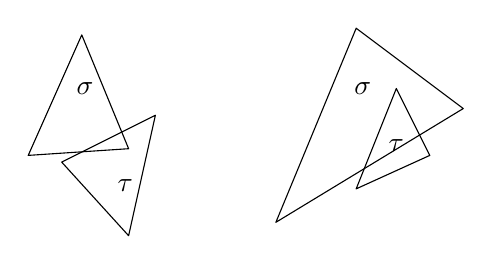
\begin{tikzpicture}[scale=.85,line cap=round,line join=round]
  \draw (-3.5,0)--(-2.7,1.8)--(-2.0,.1)--cycle;
  \draw (-3.0,-.1)--(-1.6,.6)--(-2.0,-1.2)--cycle;
  \node at (-2.65,1.0) {$\sigma$}; \node at (-2.05,-.45) {$\tau$};
  \draw (.2,-1.0)--(1.4,1.9)--(3.0,.7)--cycle;
  \draw (1.4,-.5)--(2.5,.0)--(2.0,1.0)--cycle;
  \node at (1.5,1.0) {$\sigma$}; \node at (2.0,.15) {$\tau$};
\end{tikzpicture}
\caption{不规则相处的单形}
\end{figure}

我们求积分的区域可以是复形中若干个单形组成的，但每个单形出现的次数不一定是一次，而且定向也可改变。因此我们将考虑一个“链”(chain)，即
\begin{equation}
 c=\sum_i n_i\sigma^i,\qquad n_i\text{ 为整数}.
 \tag{7}
\end{equation}
而因为一个复形中只有有限个单形，所以只有有限多个 $n_i\ne0$，而且我们规定 $\sigma^i$ 之维数相同，这个公共的维数也就成为链的维数。(7)式是一个形式和，按照形式的加法，它将构成一个可交换群。我们要求当且仅当(7)式中一切 $n_i=0$ 时，这个链才是上述群中的零元。若上述公共维数为 $k$，则称此群是一个 $k$ 维链群，记作 $C_k$。

现在把 $\partial$ 线性地由一个单形推广到链 $c$ 上，面令
\[
 \partial c=\sum_i n_i\partial\sigma^i.
\]
由(6)，$\partial\sigma^i$ 其实已经是一个链，但是维数低1，所以我们得到链群上的一个映射序列，记作 $(C,\partial)$：
\begin{equation}
 (C,\partial):\cdots\xrightarrow{\partial}C_k\xrightarrow{\partial}C_{k-1}
 \xrightarrow{\partial}\cdots\xrightarrow{\partial}C_0\xrightarrow{\partial}0.
 \tag{8}
\end{equation}
最后一项为 $0$ 是因为 $C_0$ 是由复形 $K$ 中之一切单形的顶点所成的形式和(7)之集合，顶点 $x_i$ 没有边缘，即边缘为空集，我们用 $0$ 表示空集之形式和。

\noindent\textbf{定理1}\quad $\partial^2=0$。

\noindent\textbf{证}\quad
我们只考虑一个单形 $\sigma=\langle x_0,x_1,\ldots,x_k\rangle$，则
\[
 \partial\sigma=\sum_i(-1)^i\langle x_0,\ldots,\widehat{x_i},\ldots,x_k\rangle.
\]
再施行 $\partial$ 时注意到 $\partial\sigma$ 已是一个链，而 $\partial$ 应施加于其每一项上。当 $\partial$ 施于某一项 $\langle x_0,\ldots,\widehat{x_i},\ldots,x_k\rangle$ 时应再删去一个顶点 $x_j$，如果 $j<i$，则删去的是第 $j+1$ 个顶点，应该加一个因子 $(-1)^j$；如果 $j>i$，则因 $x_i$ 本已删去，再删的是第 $j$ 个顶点，因此现在添加的因子是 $(-1)^{j-1}$。总之我们有
\begin{align*}
 \partial^2\sigma=\partial\partial\sigma
 &=\sum_{j<i}(-1)^{i+j}
 \langle x_0,\ldots,\widehat{x_j},\ldots,\widehat{x_i},\ldots,x_k\rangle\\
 &\quad+\sum_{j>i}(-1)^{i+j-1}
 \langle x_0,\ldots,\widehat{x_i},\ldots,\widehat{x_j},\ldots,x_k\rangle=0.
\end{align*}
最后一式的来源是将后一项的 $i,j$ 对调即知它与第一项和式相消。证毕。

定理1是一个非常重要的定理，它与外微分算子的基本公式 $d^2=0$ 有深刻的对偶关系。也正因为如此，我们才把可以写为 $d\sigma$ 的微分形式 $\omega=d\sigma$ 称为“上”之边缘，英文名词为 co-boundary。在数学的这一部分中，一个限制词加上了“co-”这样的字头以后总是意味着有某种对偶性。但其译法不一，有时称为“协”，如“协变”covariant，有时译为“余”，如“余切丛”cotangent bundle，有时译为“上”，如现在我们讲的“上同调”cohomology。

我们用(6)式来定义 $\partial$，其中有因子 $(-1)^i$，其目的就是为了证明这个定理。

这样，例如对 $2$ 单形 $\langle x_0,x_1,x_2\rangle$，我们有
\[
 \partial\langle x_0,x_1,x_2\rangle
 =\langle x_1,x_2\rangle-\langle x_0,x_2\rangle+\langle x_0,x_1\rangle.
\]
注意第二项 $\langle x_0,x_2\rangle$ 是由 $x_0$ 到 $x_2$ 的线段，现在要把它改成 $\langle x_2,x_0\rangle$，即由 $x_2$ 到 $x_0$ 的线段，这样做才能使一个单形的定向与它的各个面的定向协调起来（图7-5-2）。

\begin{figure}[htbp]
\centering
\begin{tikzpicture}[scale=1.0,>=stealth]
  \coordinate (A) at (0,0); \coordinate (B) at (4,0); \coordinate (C) at (2,3);
  \draw[->] (A)--($(B)!0.92!(A)$); % temporary invisible? 
  \draw (A)--(B)--(C)--cycle;
  \draw[->] (A)--(B); \draw[->] (B)--(C); \draw[->] (C)--(A);
  \node[below] at (A) {$x_0$}; \node[below] at (B) {$x_1$}; \node[above] at (C) {$x_2$};
  \draw[->] (2.1,1.35) arc[start angle=-25,end angle=270,radius=.45];
\end{tikzpicture}
\caption{$2$ 单形的边缘定向}
\end{figure}

在以前作积分时，我们要把积分中的“矩形”（第四章中通称为“区间”）细分。现在既然用单形来取代矩形，当然就要考虑单形的剖分。我们总是用一种特殊的剖分称为单形的重心重分(barycentric subdivision)。“重心”是一个从初等几何中就熟知的概念，重应读成如轻重的重。“重分”则是再分的意思，所以重分的“重”应该读如“轻舟已过万重山”的“重”。

一个 $k$ 单形 $\sigma_k=\langle x_0,x_1,\ldots,x_k\rangle$（其中 $x_i$ 表示 $n$ 维线性空间 $V$ 之一点，因此是一个 $n$ 维向量）的重心即
\begin{equation}
 b(\sigma_k)=\frac1{k+1}\sum_{i=0}^k x_i.
 \tag{9}
\end{equation}
它仍是一个 $n$ 维向量，因此仍是 $V$ 中一点，但因 $\sigma_k$ 是凸的，(9)中的系数 $\frac1{k+1}>0$，且 $\sum_{i=0}^k\frac1{k+1}=1$，所以 $b(\sigma_k)$ 在 $\sigma_k$ 内部，我们熟知的线段中点、三角形重心均是其特例。

\noindent\textbf{定义2}\quad
$\sigma_k$ 之重心重分 $D(\sigma_k)$ 即将 $\sigma_k$ 分成一切可能的以下形状的一组 $k$ 单形，其顶点为
\[
 \langle b(\tau_0),b(\tau_1),\ldots,b(\tau_k)\rangle,
\]
这里 $\tau_i$ 为 $\sigma_k$ 的一个 $i$ 维面，$b(\tau_i)$ 即其重心，而且 $\tau_i<\tau_{i+1}$。

\textbf{注意}\quad
$\tau_0$ 是 $\sigma_k$ 的 $0$ 维面即一个顶点，设为 $x_{i_0}$，$\tau_1$ 既是 $1$ 维面，面 $\tau_0<\tau_1$，所以 $\tau_1$ 必为某个线段 $[x_{i_0},x_{i_1}]$，而 $b(\tau_1)=\frac12(x_{i_0}+x_{i_1})$；同样，$b(\tau_k)=\frac1{k+1}\sum_{j=0}^k x_j$。但是从上面的作法可知，$\tau_i$ 的顶点必不能只取 $\tau_{i-1}$ 的顶点，所以 $|x_i|$ 一定是 $|x_0,x_1,\ldots,x_k|$ 的一个重新排列，而 $b(\tau_k)=b(\sigma_k)$。当然，我们应该来证明 $\langle b(\tau_0),b(\tau_1),\ldots,b(\tau_k)\rangle$ 确为一个单形。为此，只要证明它的顶点为仿射无关的即可。这是容易的。为方便起见，我们令 $\tau_j=\langle x_0,\ldots,x_j\rangle$，则
\begin{align*}
 \sum_{i=0}^k\lambda_i b(\tau_i)
 &=\sum_{i=0}^k\frac{\lambda_i}{i+1}\sum_{j=0}^i x_j\\
 &=\left(\lambda_0+\frac{\lambda_1}{2}+\cdots+\frac{\lambda_k}{k+1}\right)x_0\\
 &\quad+\left(\frac{\lambda_1}{2}+\cdots+\frac{\lambda_k}{k+1}\right)x_1
 +\cdots+\frac{\lambda_k}{k+1}x_k.
\end{align*}
若它等于 $0$，由 $\{x_0,x_1,\ldots,x_k\}$ 之仿射无关性，立即有 $\lambda_k=0$，依次代入前面各项又依次有 $\lambda_{k-1}=\lambda_{k-2}=\cdots=\lambda_0=0$。

还要注意，$\sigma_k$ 之重心重分 $D(\sigma_k)$ 一定成一复形，即它的各个小的 $k$ 维单形 $\langle b(\tau_0),b(\tau_1),\ldots,b(\tau_k)\rangle$ 均规则地相处。这在直观上是很清楚的，但是应该要证明。由于我们在这里并不是想要讨论代数拓扑学，所以不再细究这个问题了。但有一点应该提及，即在重心重分以后所得到的小的单形的定向应如何确定？从形式上看，每一个小单形 $\langle b(\tau_0),b(\tau_1),\ldots,b(\tau_k)\rangle$ 中 $\tau_i<\tau_{i+1}$，所以这些顶点已经有了一个自然的定向，但是这个定向与原来的单形之定向却不一定协调。例如，$b(\tau_0)$ 一定是某个顶点 $x_{i_0}$，$b(\tau_1)$ 应是线段 $(x_{i_0},x_{i_1})$ 的中点，但是在原单形中 $(x_{i_0},x_{i_1})$ 的定向不一定是由 $x_{i_0}$ 到 $x_{i_1}$ 而可能是相反，例如图7-5-3之左。现在我们要调整如下：我们已说过，$|i_0,i_1,\ldots,i_k|$ 一定是 $\{0,1,\ldots,k\}$ 的一个排列 $\pi$，于是我们规定小单形 $\langle b(\tau_0),b(\tau_1),\ldots,b(\tau_k)\rangle$ 的定向应取为 $\operatorname{sgn}\pi\langle b(\tau_0),b(\tau_1),\ldots,b(\tau_k)\rangle$，图7-5-3右就是调整以后的定向。

\begin{figure}[htbp]
\centering
\begin{tikzpicture}[scale=.78,>=stealth,line cap=round,line join=round]
 \begin{scope}[xshift=0cm]
   \coordinate (A) at (0,0); \coordinate (B) at (3.4,0); \coordinate (C) at (2.4,4);
   \coordinate (AB) at ($(A)!.5!(B)$); \coordinate (AC) at ($(A)!.5!(C)$); \coordinate (BC) at ($(B)!.5!(C)$);
   \coordinate (G) at (1.93,1.33);
   \draw (A)--(B)--(C)--cycle;
   \draw (A)--(G)--(B) (C)--(G) (AB)--(G) (AC)--(G) (BC)--(G);
   \node[below] at (A) {$x_0$}; \node[below] at (B) {$x_1$}; \node[above] at (C) {$x_2$};
 \end{scope}
 \begin{scope}[xshift=5.2cm]
   \coordinate (A2) at (0,0); \coordinate (B2) at (3.4,0); \coordinate (C2) at (2.4,4);
   \coordinate (AB2) at ($(A2)!.5!(B2)$); \coordinate (AC2) at ($(A2)!.5!(C2)$); \coordinate (BC2) at ($(B2)!.5!(C2)$);
   \coordinate (G2) at (1.93,1.33);
   \draw (A2)--(B2)--(C2)--cycle;
   \draw (A2)--(G2)--(B2) (C2)--(G2) (AB2)--(G2) (AC2)--(G2) (BC2)--(G2);
   \node[below] at (A2) {$x_0$}; \node[below] at (B2) {$x_1$}; \node[above] at (C2) {$x_2$};
 \end{scope}
\end{tikzpicture}
\caption{单形的重心重分与定向调整}
\end{figure}

我们当然要对 $\sigma$ 反复作重心重分，例如作出 $D^m(\sigma)=D\cdot D\cdots D(\sigma)$（共 $m$ 重），而看 $m\to\infty$ 时它是否会缩为一点。这时就要问了，在 $V$ 上我们并未赋以度量，怎样来考虑极限呢？事实上，$V\cong\mathbb R^n$，在 $\mathbb R^n$ 中当然可以作出极限，当然可以给出度量（见第六章）而不必要有欧氏度量（这一点与体积不同，要定义体积却是需要欧氏度量的）。而且第六章中还指出了，$\mathbb R^n$ 中各种度量均是等价的。例如两个点 $x_1=(x_1^1,\ldots,x_1^n)$ 与 $x_2=(x_2^1,\ldots,x_2^n)$ 之间，用 $\sum_i|x_1^i-x_2^i|$，$\sup_i|x_1^i-x_2^i|$，$[\sum_i(x_1^i-x_2^i)^p]^{1/p}(p>1)$ 作距离均无不可，所以以下面我们直接写 $|x-y|$ 表示二点的距离。于是令 $\sigma=\langle x_0,x_1,\ldots,x_k\rangle$ 为一个单形，$x,y\in\sigma$，于是 $y=\sum_{i=0}^k\lambda_i x_i,0\le\lambda_i\le1,\sum\lambda_i=1$，所以
\[
 |x-y|\le\sum_{i=0}^k\lambda_i|x-x_i|
 \le\sup_i|x_i-x|\le\sup_{i,j}|x_i-x_j|.
\]
这里我们再把 $x$ 写为 $x=\sum_{j=0}^k\mu_jx_j$，然后再用上面的推理。作重心重分后，我们只要讨论 $|b(\tau)-b(\mu)|$ 即可。于是设 $\tau<\mu$，$b(\tau)$ 是一个 $l$ 维面的重心，$b(\mu)$ 是一个 $m$ 维面的重心，$l<m\le k$，于是
\[
 b(\tau)=\frac1{l+1}\sum_{i=0}^l x_i,
 \qquad
 b(\mu)=\frac1{m+1}\sum_{j=0}^m x_{i_j}.
\]
为了避免符号过于冗长，$x_{i_j},x_{i'_j}$ 就写成 $x_j,x_{j'}$，这样利用单形为一个凸集，即知
\begin{align*}
 |b(\tau)-b(\mu)|
 &\le \sup_j|x_j-b(\mu)|\\
 &\le \sup_{i,j}\left|x_j-\frac1{m+1}\sum_{i=0}^m x_{i'}\right|\\
 &\le \sup_{i,j}\left|\frac1{m+1}\sum_{i=0}^m(x_j-x_{i'})\right|\\
 &\le \frac{m}{m+1}\sup_{i,j}|x_i-x_j|
 \le \frac{k}{k+1}(\sigma\text{ 之直径}).
\end{align*}
由此可知，当无限地作重心重分后，单形 $\sigma$ 将缩为一点。

有了这些预备知识以后，我们可以开始讨论积分了。我们首先考虑一个 $k$ 形式 $\omega=a(x)dx^1\wedge\cdots\wedge dx^k$ 在一个 $k$ 单形 $\sigma_k=\langle x_0,x_1,\ldots,x_k\rangle$ 上的积分。这里遇到了关键问题，即如何处理体积。如果在 $\mathbb R^n$ 上已有欧氏结构，而且不妨即设 $(x^1,\ldots,x^k)$ 为笛卡尔坐标，则切空间有一个 o.n. 基底 $\{e_1,\ldots,e_k\}=\{\partial/\partial x^1,\ldots,\partial/\partial x^k\}$，$\{dx^1,\ldots,dx^k\}$ 则是余切空间与它对偶的 o.n. 基底。如果记 $\sigma_k$ 之棱为切向量 $\{v_1,\ldots,v_k\}$（实际上例如 $v_1=x_1-x_0$），而且
\[
 v_i=A_i^{\ j}\frac{\partial}{\partial x^j}
 \qquad(\text{注意 }A_i^{\ j}\text{ 为实常数}),
\]
于是 $dx^1\wedge\cdots\wedge dx^k$ 作为 $k$ 阶反对称协变张量，易知
\begin{align*}
 &\langle dx^1\wedge\cdots\wedge dx^k;v_1,\ldots,v_k\rangle\\
 &\qquad=\det(A_i^{\ j})
 \langle dx^1\wedge\cdots\wedge dx^k;
 \partial_{x^1},\ldots,\partial_{x^k}\rangle\\
 &\qquad=\det(A_i^{\ j})=k!\operatorname{vol}(\sigma_k).
\end{align*}
今取 $\omega$ 之系数 $a(x)$ 在 $\sigma_k$ 的重心 $b_k$ 处的值 $a(b_k)$，并且作出第一个“黎曼和”
\begin{equation}
\begin{aligned}
 S_1(\omega,\sigma_k)
 &=\frac1{k!}\langle a(b_k)dx^1\wedge\cdots\wedge dx^k;
 v_1^{(1)},\ldots,v_k^{(1)}\rangle\\
 &=a(b_k)\operatorname{vol}(\sigma_k).
\end{aligned}
 \tag{10}
\end{equation}
这里 $v_i^{(1)}$ 就是 $v_i$。(10)式前的因子 $1/k!$ 来自：$\det(A_i^{\ j})$ 是 $k$ 维平行体的有符号的体积，乘上 $1/k!$ 后才得到单形 $\sigma_k$ 的体积 $\operatorname{vol}(\sigma_k)$。

往下的作法就很清楚了。作 $\sigma_k$ 的二次重分 $D^2(\sigma_k)$。它是一个链，由具有适当符号的 $k$ 单形 $\sigma_{k,i}^{(2)}$ 构成。对每个这样的单形，仿照(10)作出
\begin{align*}
 S_2(\omega,\sigma^{(2)})
 &=\frac1{k!}\sum_i\langle a(b_{k,i}^{(2)})dx^1\wedge\cdots\wedge dx^k;
 v_1^{i(2)},\ldots,v_k^{i(2)}\rangle\\
 &=\sum_i a(b_{k,i}^{(2)})\operatorname{vol}(\sigma_{k,i}^{(2)}).
\end{align*}
然后再作出
\begin{equation}
\begin{aligned}
 S_m(\omega,\sigma^{(m)})
 &=\frac1{k!}\sum_i\langle a(b_{k,i}^{(m)})dx^1\wedge\cdots\wedge dx^k;
 v_1^{i(m)},\ldots,v_k^{i(m)}\rangle\\
 &=\sum_i a(b_{k,i}^{(m)})\operatorname{vol}(\sigma_{k,i}^{(m)}).
\end{aligned}
 \tag{11}
\end{equation}
我们考虑的是 $\mathbb R^k$ 上的光滑微分形式，所以应该看到 $a(x)$ 在有界闭集 $\sigma_k$ 上是连续的，因而是黎曼可积的，因此当 $m\to\infty$ 时，$\lim_{m\to\infty}S_m(\omega,\sigma^{(m)})=\int_{\sigma_k}a(x)dx^1\cdots dx^k$ 是存在的。所以，我们有理由给出

\noindent\textbf{定义3}\quad
若 $\omega=a(x)dx^1\wedge\cdots\wedge dx^k$ 在 $\mathbb R^k$ 中包含某个 $k$ 维单形 $\sigma_k$ 的区域中是光滑的 $k$ 形式，则定义
\begin{equation}
 \int_{\sigma_k}\omega=\int_{\sigma_k}a(x)dx^1\cdots dx^k.
 \tag{12}
\end{equation}

对这个定义应该作一些说明。在定义3前的一大段文字并没有证明什么，而只是解释为什么要这样定义。古典的积分定义的主要思想，如果给以不严格的表述，就是：把一个函数 $a(x)$，乘上“无穷小的体积”$dx^1\cdots dx^k$，再加起来。现在则是，把一个微分形式 $\omega$ 中的“体积元素”$dx^1\wedge\cdots\wedge dx^k$ 作用到“无穷小单形”$\sigma_{k,i}^{(m)}$ 上并乘以 $a(b_{k,i}^{(m)})$，然后再加起来，二者实在是很相似的。问题在于 $\mathbb R^k$ 上本没有给出度量以前，是不能定义体积的。$\mathbb R^k$ 上当然可以给出度量，而且可以给出许多种；每一个度量就是一个正定的 $k$ 阶方阵 $(g_{ij})$。上面的讲法则是指定用单位矩阵 $I$ 作为 $(g_{ij})$。当然会问，如果给出其它度量又当如何？结果当然会有所不同，下面讲到函数（而不是微分形式）在黎曼流形（上面当然已经有了度量）上的积分时会要回答这个问题。可以说其结果无非相当于对系数 $a(x)$（即“被积函数”）作一个修正而已。这时整个理论不会有本质的改变。但它完整告诉我们，微分形式的积分本质上依赖于体积概念，体积是可以“定义”的。用不同定义的体积将得到不同的积分值。真正的问题是：$\mathbb R^k$ 上本来没有体积，要先给出体积定义以后，才能用这样算出的黎曼积分 $\int a(x)dx^1\cdots dx^k$ 作为 $\int\omega$ 之定义。

我们的作法当然有些偷巧。既然知道 $dx^1\wedge\cdots\wedge dx^k$ 作用到 $(v_1,\ldots,v_k)$ 上以后可以得到一个“很像”体积的东西，何不以它为基础建立一套测度和积分理论而要将它归结为通常的黎曼积分呢？如果那样做就太麻烦了。回想一下古典的黎曼积分定义是很麻烦的（二维情况好说，到了三维一定要考虑高维问题），在高维时，我们需要把积分区域分解成若干当可测的小区域（而什么条件下一个区域才是若尔当可测又是麻烦事）。现在我们只分划为单形，而单形又只允许作重心重分，这当然容易多了。特别是把它化成了黎曼积分就不必操心证明这个“很像”体积的东西是否具有有限或可数可加性了。可是以单形及其重心重分为基础来建立积分理论真正的目的是为了突出积分的组合学的侧面，表现在下面的斯托克斯定理上。

根据同样的“偷巧”的办法，有许多关于积分必须要证明的结果将都在其较一般的情况下，即流形上的积分中，一并证明。

最后还要提一下，我们的 $\operatorname{vol}(\sigma_k)$ 是有符号的：若将 $\sigma_k$ 的定向反转，成为 $-\sigma_k$ 则 $\det(A_i^{\ j})$ 将要反号，于是
\begin{equation}
 \int_{-\sigma_k}\omega=-\int_{\sigma_k}\omega.
 \tag{13}
\end{equation}
这可能是微分形式的积分与通常函数的积分最重要的区别。也很清楚，若有一个由 $k$ 单形 $\sigma_k^{(i)}$，$i=1,2,\ldots,l$（$l$ 为有限整数）所成的链
\begin{equation}
 c=\sum_{i=1}^l\lambda_i\sigma_k^{(i)},\qquad \lambda_i\in\mathbb Z,
 \tag{14}
\end{equation}
（这里 $\mathbb Z$ 指整数集），则可以在链上求积分而有
\begin{equation}
 \int_c\omega=\sum_{i=1}^l\lambda_i\int_{\sigma_k^{(i)}}\omega.
 \tag{15}
\end{equation}

\noindent\textbf{2. 斯托克斯定理}\quad
许多数学家认为斯托克斯定理是整个数学中最深刻的定理之一。其实，在19世纪中叶有许多类似的定理都差不多同时被人提出，例如高斯、格林的定理。对之有贡献的数学家与数学物理学家还可以举出许多，它之所以重要在于它几乎是自明的，而这又依赖于彻底地弄清楚它所涉及的概念。同时它有十分重要的推论。由于它十分重要，我们宁可多花一些篇幅，在 $\mathbb R^n$ 上与在一般的微分流形上各讲一次，这样可以更清楚地理解它所涉及的概念。

\noindent\textbf{斯托克斯定理}\quad
设 $\sigma$ 为一有向 $k$ 维单形，$\omega$ 为 $\sigma$ 上的光滑的 $(k-1)$ 微分形式，则
\begin{equation}
 \int_\sigma d\omega=\int_{\partial\sigma}\omega.
 \tag{16}
\end{equation}

\noindent\textbf{证}\quad
我们最终将在一个微分流形上证明类似定理，那时我们也将给出其准确的提法。所以现在我们仍只限于说明，从组合学的角度去看，它究竟是怎么回事。

上面我们说过，若 $\sigma=\langle x_0,x_1,\ldots,x_k\rangle$ 则
\[
 \partial\sigma=\sum_{i=0}^k(-1)^i\langle x_0,\ldots,\widehat{x_i},\ldots,x_k\rangle.
\]
我们看左、右双方的黎曼和，而且首先起 $\sigma$ 未作重心重分的情况。对于(16)的左方，它是
\[
 S_1(d\omega,\sigma)=\frac1{k!}\langle d\omega|_{x=b(\sigma)};v_1,\ldots,v_k\rangle.
\]
但是上一节中的(21)式（我们只对 $\omega$ 为1微分形式的情况证明了它）告诉我们
\[
 \langle d\omega|_{x=b(\sigma)};v_1,\ldots,v_k\rangle
 =\sum_{j=1}^k(-1)^{j-1}D_{v_j}\langle\omega;v_1,\ldots,\widehat{v_j},\ldots,v_k\rangle|_{x=b(\sigma)}+\text{其它项}.
\]
这里“其它项”形如 $\langle\omega(b(\sigma));[v_i,v_j],v_1,\ldots,\widehat{v_i},\ldots,\widehat{v_j},\ldots,v_k\rangle$，而且 $D_{v_i}$ 就表示在 $v_i$ 方向的方向导数，亦即(9)式中的 $v_i=A_i^{\ j}\frac{\partial}{\partial x^j}$。但是 $v_i$ 都是常系数微分算子，因此互相间都可以交换：$[v_i,v_j]=0$，因此“其它项”是不会出现的。故
\begin{equation}
 S_1(d\omega,\sigma)
 =\frac1{k!}\sum_{j=1}^k(-1)^{j-1}D_{v_j}
 \langle\omega(b(\sigma));v_1,\ldots,\widehat{v_j},\ldots,v_k\rangle.
 \tag{17}
\end{equation}
再看(16)的右方，相应于它的黎曼和是
\[
 S_1(\omega,\partial\sigma)=\frac1{(k-1)!}\sum_{j=0}^k(-1)^jS_1(\omega,\sigma_j).
\]
$\sigma_j=\langle x_0,\ldots,\widehat{x_j},\ldots,x_k\rangle$，当 $j>0$ 时它是由 $\{v_1,\ldots,\widehat{v_j},\ldots,v_k\}$ 构成的 $(k-1)$ 单形。但是当 $j=0$ 时 $\sigma_0=\langle x_1,\ldots,x_k\rangle$ 的棱是 $\{w_i=x_i-x_1=v_i-v_1\},i=2,\ldots,k$。因此在 $S_1(\omega,\sigma_0)$ 中 $\omega$ 是作用于 $w_2\wedge\cdots\wedge w_k=(v_2-v_1)\wedge\cdots\wedge(v_k-v_1)$ 的。把 $w_2\wedge\cdots\wedge w_k$ 按 $v_1$ 展开，其第一项不含 $v_1$ 而是 $v_2\wedge\cdots\wedge v_k$；含 $v_1$ 的“一次幂”若是在 $(v_2,\ldots,v_j,\ldots,v_k)$ 中以 $-v_1$ 代替 $v_j$，其它项则至少含两个 $v_1$ 作为因子，外微分形式 $\omega$ 既是反对称协变张量，则它作用于含两个（或更多）相同因子 $v_1$ 的项上自然为0，因此
\begin{align}
 S_1(\omega,\partial\sigma)
 &=\frac1{(k-1)!}\left\{(-1)^0S_1(\omega(b_0),\sigma_0)+\sum_{j=1}^k(-1)^j\langle\omega(b_j),\sigma_j\rangle\right\}\notag\\
 &=\frac1{(k-1)!}\sum_{j=1}^k(-1)^j\langle\omega(b_j),v_1,\ldots,\widehat{v_j},\ldots,v_k\rangle\\
 &\quad+\frac1{(k-1)!}\sum_{j=1}^k(-1)^{j-1}\langle\omega(b_0),v_1,\ldots,\widehat{v_j},\ldots,v_k\rangle.
 \tag{18}
\end{align}
这两项不同在于，第二项中是在 $b_0$ 处取 $\omega$ 之值，而第一项则是在 $\sigma$ 之第 $j$ 个面 $\sigma_j$ 之重心 $b_j$ 处取 $\omega$ 之值。所以
\[
 S_1(\omega,\partial\sigma)
 =\frac1{(k-1)!}\sum_{j=1}^k(-1)^{j-1}
 \langle[\omega(b_0)-\omega(b_j)],v_1,\ldots,\widehat{v_j},\ldots,v_k\rangle.
\]
下面是关键的一步。应用中值定理于 $\omega(b_0)-\omega(b_j)$。在微分学一章中我们就指出过，对于多元函数，中值定理一般不成立，而只能用一个不等式来代替。现在注意单形 $\sigma$ 对其任何一点都是星形的，因此连接 $b_0$ 与 $b_j$ 的线段 $\{tb_0+(1-t)b_j,0\le t\le1\}$ 恒在 $\sigma$ 内，而 $\omega$ 在这个线段上确实是单变量 $t$ 的函数，因此可以应用中值定理（更准确地说是应用专用于一元函数的拉格朗日公式）而知在此线段上一定可以找到一点 $c_j$，使
\[
 \omega(b_0)-\omega(b_j)=D_{v_j}(c_j)(b_0-b_j).
\]
这里 $D_{v_j}$ 是沿 $(b_0,b_j)$ 线段的方向导数，而因
\[
 b_0-b_j=\frac1k\left(\sum_{i\ne0}x_i-\sum_{i\ne j}x_i\right)
 =\frac1k(x_j-x_0)=\frac1k v_j,
\]
所以就是 $v_j$ 方向的向量，从而
\[
 \omega(b_0)-\omega(b_j)=\frac1kD_{v_j}(c_j)v_j.
\]
代入(18)即有
\begin{equation}
 S_1(\omega,\partial\sigma)
 =\frac1{k!}\sum_{j=1}^k(-1)^{j-1}
 D_{v_j}\langle\omega(c_j),v_1,\ldots,\widehat{v_j},\ldots,v_k\rangle.
 \tag{19}
\end{equation}
把(17)与(19)比较，其差别一是在 $c_j$ 处求值，一是在 $b(\sigma)$ 处求值。但在经过多次重心重分后 $b(\sigma)$ 与 $c_j$ 会任意接近，而且若以重心重分后 $k$ 维单形之直径作为无穷小量之阶的标准，则每一项之差均为高阶无穷小量。按照黎曼积分的标准作法，其极限又会相同。由此即得斯托克斯定理之证。

认真分析这个证明，首先我们应看到这个定理是微积分基本定理的推广。因为若 $\sigma$ 是1维单形即区间 $[x_0,x_1]$ 时，$\omega$ 应是0形式，即一个 $C^\infty$ 函数 $f(x)$，$d\omega=f'(x)dx$，而 $\omega$ 在 $\partial\sigma=\{x_1\}-\{x_0\}$ 上的“积分”现在成为 $f(x_1)-f(x_0)$，斯托克斯定理就成了
\[
 \int_{x_0}^{x_1}f'(x)dx=f(x_1)-f(x_0).
\]
当然读者会说，这里对 $f(x)$ 光滑性要求过高，整个第四章可以说正是围绕可积性而来，那么何必那么大张旗鼓地讲斯托克斯定理是它的推广呢？大凡一个重要理论总有许多不同的侧面。以定积分为例，它的积分区域构造极为简单，可是古代不明白什么叫可积性。到柯西解决了连续函数的积分问题以后，不连续性问题提到议事日程上来。由黎曼、达布等又提出了可积性的理论。后来出现了勒贝格的理论，我们在第四章中正是这样展开这个理论的。可是这只是问题的一个侧面。当我们看到，特别是在物理学中的曲线积分与曲面积分，其积分区域的几何构造（准确些说是其拓扑特性）变得十分复杂时，就发现微分流形上的微分形式之积分成了不可避免的对象。这时，研究积分的几何、拓扑侧面就自然凸现出来。而斯托克斯定理就自然成了人们注意的中心。法国大数学家托姆(R. Thom)说过一段话：“要问我最深刻、最困难而又有具体的不容置疑的物理解释的数学定理是哪一个？对于我，斯托克斯定理当属首选。这与下面的事实有关：外微分是一个十分神秘的观念，它的真正的实质，我相信，还藏在谜中，尽管它的形式定义是如此简单。”（转引自 D. Leborgne, Calcul différentiel et géométrie, 1982, 146页）。

在上述证明中最令人注意的是什么？一是中值定理的应用。从我们在第四章 §1 中介绍的达布关于微积分基本定理的证明中，我们就看见这个定理的作用，在讲到泰勒展开式的积分余项时，也是利用 $x$ 点与 $x_0$ 点的连线当 $x$ 与 $x_0$ 充分接近，全部落在所考虑的区域内，因而可以利用积分中值定理（也就是拉格朗日公式）。在庞加莱引理和这里则明确提出了区域的星形的概念。它与在拓扑学上重要的可收缩性概念相关。我们要指出，在许多其它重要定理中，也都会以类似形式应用中值定理。二是组合方法的应用，即在本书中这也不是第一次了：达布对微积分基本定理的证明就是利用了一个极其简单的组合学事实：
\[
 F(b)-F(a)=F(a_N)-F(a_0)=\sum_{i=1}^N[F(a_i)-F(a_{i-1})].
\]
我们也指出过，分部积分法，无非就是连续形式的阿贝尔求和变换式
\[
 \sum_{k=1}^N(a_k-a_{k-1})b_k
 =\sum_{k=0}^N(b_k-b_{k+1})a_k,\qquad a_0=b_{N+1}=0.
\]
现在斯托克斯定理的证明，以及它的基础：单形的边缘与复形的边缘计算公式中的符号的选取，都是使用了组合学的技巧，其目的在于正负相消得到十分简洁的结果。我们在前面说积分学还有另一个侧面即组合学的侧面，就是这个意思。当然，积分学不止是一点组合学，还有“一点”逼近，“一点”极限。其实，这里讲的“一点”也都会成为大文章，下面还要再说。现在我们想告诉读者的是这样一个事实：贯串在整个数学中有一些最基本、最简单的思想和方法。但是它们变化万千，丰富多采。我们学好一门学问，最要下力气的正是用一切方法掌握这些为数不多的基本思想、基本方法，以达到返朴归真。可是没有多年独立的钻研，这是绝做不到的。

\noindent\textbf{3. 微分形式在流形上的积分以及一般的斯托克斯定理}\quad
本节中我们恒设 $M$ 是一个 $n$ 维可定向微分流形。

微分流形上的积分理论有两个最重要之点：其一是这个理论应该是与坐标无关的，其二是斯托克斯定理。第一点我们在一开始就提到了，它其实就是坐标变换公式，它可以由式(1)，即
\[
 \int_U\omega=\int_V\varphi^*\Omega=\int_{\varphi(U)}\Omega
\]
得出。如果 $U$ 是 $\mathbb R^n$ 中的一个复形，$\varphi(U)$ 在 $M$ 上，$M$ 是弯曲的，其上本来没有平直的单形和复形，是否可以设想，$\varphi$ 把复形的结构映射到 $M$ 上，即将 $M$ 分成许多小块，每一个小块 $U_i$ 是一个 $n$ 维单形 $\sigma$ 之像，而 $\sigma$ 之面，分别映射到 $U_i$ 的一个低维子流形上？如果可以，就称 $U\subset M$ 是一个 $k$ 维奇异单形。称它为奇异的是因为由 $\sigma$ 到 $U$ 的映射 $\varphi$ 允许很“奇异”，甚至不一定是一对一的。这些奇异单形的形式和 $\sum_i\sigma_i$ 称为奇异链。如果存在这样的一个映射，就说 $M$ 可以三角剖分。如果这个映射是 $C^\infty$ 的则说 $M$ 可以 $C^\infty$ 地三角剖分。那么，$M$ 是否可以 $C^\infty$ 三角剖分呢？从20世纪30年代起这就是一个重大问题，因为它关系到能否把组合的方法用于微分流形的研究。这里有惠特尼(Hassler Whitney)的三角剖分定理，指出每一个 $C^\infty$ 微分流形一定有 $C^\infty$ 三角剖分。这个定理的证明太复杂，不妨留待读者有志于更深入地讨论流形的拓扑学时再去研讨。现在我们用另一种方法来讨论，这就是应用单位分解。

在微分流形 $M$ 的定义中我们加上了 $M$ 为豪斯多夫空间并且适合第二可数性公理的要求（§2），那时我们就指出这样做是为了使用单位分解。其实前面我们已经多次这样做了，现在再比较明确地讲一下定义积分的过程，它是应用单位分解方法的一个典型例子。所谓单位分解就是：在上述关于 $M$ 的限制下，若 $M$ 有一个开覆盖，则它必有一个局部有限的子覆盖 $\{U_\alpha\}$，即每一点 $P$ 必有一个邻域 $W$，与最多有限多个 $U_\alpha$（设为 $U_1,\ldots,U_k$）相交：$U_i\cap W\ne\varnothing,i=1,2,\ldots,k$，然后可以找到一族 $C^\infty(M)$ 函数 $\varphi_\alpha$，称为从属于此覆盖的单位分解，使每一个 $\varphi_\alpha$ 的支集 $\operatorname{supp}\varphi_\alpha$ 必含于某一个 $U_\beta$ 中，$\beta=\beta(\alpha)$（不说是含于 $U_\alpha$ 中，因为 $\{U_\beta\}$ 不一定与 $\{\varphi_\alpha\}$ 用同样的参数标记，而且同一个 $\operatorname{supp}\varphi$ 可以含于好几个不同的 $U_\beta$ 中，我们选定其中一个并记为 $\beta(\alpha)$），这些函数的支集 $\{\operatorname{supp}\varphi_\alpha\}$ 一定是局部有限的，而且
\begin{equation}
 0\le\varphi_\alpha\le1,\qquad \sum_\alpha\varphi_\alpha=1.
 \tag{20}
\end{equation}
后一式要注意，因为有局部有限性的要求，每一点 $P$ 至多含于有限多个 $\operatorname{supp}\varphi_\alpha$ 中，所以上式形式上看来是无限和，其实在 $M$ 之每一点上都是有限和。

现在我们讨论具有紧支集的 $n$ 微分形式 $\omega$ 在 $M$ 上的积分。限制 $\omega$ 具有紧支集的作用如何在黎曼积分中避免反常积分。实际上，令上述 $\{U_\alpha\}$ 是 $M$ 上的局部坐标邻域系，作从属于它的单位分解 $\{\varphi_\alpha\}$，于是由(20)有
\begin{equation}
 \omega=\sum_\alpha\varphi_\alpha\omega=\sum_\alpha\omega_\alpha.
 \tag{21}
\end{equation}
而且因为 $\operatorname{supp}\omega$ 为紧，它最多与有限多个 $\operatorname{supp}\varphi_\alpha$ 相交，因此上式确实是一个有限和。其每一项可以写为
\begin{equation}
 \omega_\alpha=a_\alpha(x)dx^1\wedge\cdots\wedge dx^n,
 \tag{22}
\end{equation}
$(x^1,\ldots,x^n)$ 是 $U_\alpha$ 中的局部坐标，而 $a_\alpha(x)$ 不妨认为是定义在整个 $\mathbb R^n$ 上的，只不过在 $V_\alpha=\varphi_\alpha^{-1}(U_\alpha)\subset\mathbb R^n$（$\varphi_\alpha$ 是 $U_\alpha$ 中的坐标映射）之外 $a_\alpha(x)=0$。这样 $a_\alpha(x)\in C_0^\infty(\mathbb R^n)$，这个函数的黎曼积分没有一点困难。

于是我们得到了 $\mathbb R^n$ 上的 $n$ 微分形式，其积分是可以定义的，当然要对 $\mathbb R^n$ 赋以典则的，即标准的欧氏度量。对(21)式之每一项作类似处理后，即可看出，应有

\noindent\textbf{定义4}\quad
设 $M$ 是一个可定向的 $n$ 维微分流形，$\omega$ 是 $M$ 上的一个具有紧支集的 $n$ 微分形式，则我们定义 $\omega$ 在 $M$ 上的积分为
\begin{equation}
 \int_M\omega=\sum_\alpha\int_M\omega_\alpha
 =\sum_\alpha\int_{\mathbb R^n}a_\alpha(x)dx^1\cdots dx^n.
 \tag{23}
\end{equation}
与定义3比较，在那里我们并未假设 $\omega$ 具有紧支集，但是积分域是一个单形 $\sigma_k$ 或者是有限个单形所成的链，因而是紧的。这也是为了避免反常积分那样的困难。

为了说明这个定义的合理性应该回答两个问题：首先，若采用不同的单位分解；其次，若对同一个 $\omega_\alpha$ 采用不同的局部坐标系，所得到的结果是否一致？若不一致，则这个定义是不合理的。

第一个问题很容易回答。因为若有另一个可能是从属于另一个局部有限覆盖的单位分解 $\{\psi_\beta\}$，$0\le\psi_\beta\le1,1=\sum_\beta\psi_\beta$，则应定义
\[
 \int_M\omega=\sum_\beta\int_M\psi_\beta\omega.
\]
但是
\begin{align*}
 \int_M\omega
 &=\sum_\alpha\int_M\varphi_\alpha\omega
 =\sum_\alpha\left[\sum_\beta\int_M(\varphi_\alpha\psi_\beta)\omega\right]\\
 &=\sum_\beta\left[\sum_\alpha\int_M(\psi_\beta\varphi_\alpha)\omega\right]
 =\sum_\beta\int_M\psi_\beta\left(\sum_\alpha\varphi_\alpha\omega\right)
 =\sum_\beta\int_M\psi_\beta\omega.
\end{align*}
所以采用不同的单位分解并不影响定义。

其次，若在积分区域中 $U_\alpha$ 中有两个局部坐标系 $(V,\varphi)$ 与 $(W,\psi)$，$V=\varphi^{-1}(U_\alpha),W=\psi^{-1}(U_\alpha)$，而且局部坐标分别为 $(x^1,\ldots,x^n)$ 与 $(y^1,\ldots,y^n)$，则有微分同胚 $\phi:V\to W,x=\phi(y)$，而 $\omega_\alpha$ 有两个表达式
\[
 \omega_\alpha=a_\alpha(x)dx^1\wedge\cdots\wedge dx^n
 =A_\alpha(y)dy^1\wedge\cdots\wedge dy^n,
\]
\[
 a_\alpha(x)=A_\alpha(y)\frac{\partial(y^1,\ldots,y^n)}{\partial(x^1,\ldots,x^n)}.
\]
因为我们已设 $M$ 是可定向的，当然可以要求所有的局部坐标的定向是相协调的，因此
\[
 \frac{\partial(y^1,\ldots,y^n)}{\partial(x^1,\ldots,x^n)}>0.
\]
于是
\begin{align*}
 \int\omega_\alpha
 &=\int a_\alpha(x)dx^1\cdots dx^n
 =\int A_\alpha(y)\left|\frac{\partial(y^1,\ldots,y^n)}{\partial(x^1,\ldots,x^n)}\right|dx^1\cdots dx^n\\
 &=\int A_\alpha(y)dy^1\cdots dy^n
 =\int A_\alpha(y)dy^1\wedge\cdots\wedge dy^n.
\end{align*}
正如本节一开始时就强调指出的，我们要讨论微分形式而不是函数在流形上的积分，正是因为微分形式在局部坐标下的表达式自动地含有我们所需要的变量变换公式，而假设 $M$ 是可定向的就可以保证雅可比行列式中自动地会出现绝对值。

有了定义4以后，关于流形 $M$ 上的积分之性质，有

\noindent\textbf{定理2}\quad
若以下的 $n$ 微分形式均在可定向 $n$ 维流形 $M$ 上具有紧支集，或 $M$ 为紧流形，则

(1) $\displaystyle \int_M(\lambda_1\omega_1+\lambda_2\omega_2)=\lambda_1\int_M\omega_1+\lambda_2\int_M\omega_2$，$\lambda_1,\lambda_2$ 为实数；

(2) 若将 $M$ 上定向反转，记所得流形为 $-M$，则
\begin{equation}
 \int_{-M}\omega=-\int_M\omega.
 \tag{24}
\end{equation}
证明很简单，现在均略去，不过要说明，它们对 $\mathbb R^n$ 上的积分也都成立。

这里我们要对(24)式多说几句。通常的微积分教本中讲曲线积分与曲面积分时，总分成第一型与第二型两种，其实所谓“第二型”就是在一维流形（曲线）或二维流形（曲面）上积分。在那里我们是说函数的积分，现在则应该说是微分形式 $Pdx+Qdy+Rdz$ 或 $Pdy\wedge dz+Qdz\wedge dx+Rdx\wedge dy$ 的积分（前者是曲线积分，后者是曲面积分）。不过曲面积分我们是写成 $Pdy\wedge dz+Qdz\wedge dx+Rdx\wedge dy$。第二型曲线积分适合(24)是人们都明白的：
\[
 \int_{AB}Pdx+Qdy+Rdz=-\int_{BA}Pdx+Qdy+Rdz.
\]
对曲面积分我们则说在此曲面的这一侧或另一侧积分，而单侧曲面如莫比乌斯带上是否可以积分则不涉及。其实这里也一样，我们只讨论可定向流形上的积分。不可定向流形上如何积分是另一个理论的内容。通常微积分教本中讲曲面的侧时例如是说：在曲面上指定一侧，如果我们头向这一侧站立，则在此曲面上规定逆时针方向为正向；另一侧就是，如果头向下倒立时看见的逆时针方向为正向，所以两侧有相反的定向。之所以可以这样做是因为我们承认曲面是在三维空间（即其包含空间）中的，所以有头向上、向下之说。现在的流形 $M$ 则没有包含空间，所以无所谓“侧”，要规定其中的正向，就要规定好流形之定向。不过我们有时仍借用“侧”的说法，而把(24)式说成是在 $M$ 之不同侧上的积分反号。至于第一型线积分和曲面积分，只不过是采用弧长或曲面面积 $ds,d\sigma$ 作为测度，它们都是正的，这与前面讲的黎曼或勒贝格多重积分是一样的，所以没有与(24)相应的性质。也可以说，本书前面讲的多重积分是“第一型”的，但是定积分 $\int_a^bf(x)dx$ 却是第二型的，因为它有与(24)一样的性质。

本节一开始我们就指出了微分流形上的积分定义必须是与坐标的选择无关的。因此，积分中变量变换公式起了根本的作用，其实这个公式是一个更一般的定理的特例。设有两个 $n$ 维微分流形 $M$ 和 $N$ 以及一个微分同胚 $\varphi:M\to N$，若 $\omega$ 是 $N$ 上的一个具有紧支集的 $n$ 微分形式，则它在 $M$ 上的拉回：$\varphi^*\omega$ 是 $M$ 上的一个 $n$ 微分形式，而且也具有紧支集。这时，我们有

\noindent\textbf{定理3}\quad
若 $\varphi,M,N$ 均如上述，则
\begin{equation}
 \int_M\varphi^*\omega=\varepsilon\int_{\varphi(M)}\omega.
 \tag{25}
\end{equation}
这里 $\varepsilon=\pm1$ 视 $\varphi$ 为保持定向或反转定向而定。

\noindent\textbf{证}\quad
在必要时引用上面所说的单位分解，我们可以设 $C=\operatorname{supp}\omega\subset U$，$U$ 是 $N$ 上一个坐标邻域，而坐标映射 $f:U\to\mathbb R^n$，$f(C)\subset f(U)$ 中的局部坐标为 $(y^1,\ldots,y^n)$，使得
\[
 \omega=a(y^1,\ldots,y^n)dy^1\wedge\cdots\wedge dy^n.
\]
不失一般性，可以设 $\varphi^{-1}(U)$ 在 $M$ 的一个坐标邻域中，其局部坐标是 $(x^1,\ldots,x^n)$。于是
\[
 \varphi^*\omega=A(x^1,\ldots,x^n)dx^1\wedge\cdots\wedge dx^n,
\]
而且
\[
 A(x^1,\ldots,x^n)=a(y^1,\ldots,y^n)\frac{\partial(y^1,\ldots,y^n)}{\partial(x^1,\ldots,x^n)}
 =\varepsilon a(y^1,\ldots,y^n)\left|\frac{\partial(y^1,\ldots,y^n)}{\partial(x^1,\ldots,x^n)}\right|.
\]
所以
\begin{align*}
 \int\varphi^*\omega
 &=\int A(x)dx^1\cdots dx^n\\
 &=\varepsilon\int a(y)\left|\frac{\partial(y)}{\partial(x)}\right|dx^1\cdots dx^n\\
 &=\varepsilon\int a(y)dy^1\cdots dy^n
 =\varepsilon\int\omega.
\end{align*}
必要时应用单位分解就可得到(25)。

在上面的证明中，$M$ 与 $N$ 是可定向的是一个重要条件。因为不然的话，$\varepsilon$ 可能在不同坐标邻域上不同。但是退一步说，还得 $M$ 与 $N$ 都是连通的，否则在不同的连通分支上 $\varepsilon$ 可能各取 $+1$ 或 $-1$ 而不同。这些都是很容易理解的。重要的是要明白 $\varphi$ 为微分同胚是一个本质的要求，否则的话(25)会不成立，而要改为
\[
 \int_M\varphi^*\omega=\varepsilon\deg\varphi\int_{\varphi(M)}\omega.
\]
这里的 $\deg\varphi$ 是一个整数，称为映射度(degree of mapping)。粗略地说，就是 $N$ 被 $\varphi(M)$ 覆盖的次数。其实在前面讲到微分形式的拉回时，就出现了这个问题，不过我们没有深究。

如果 $M=N$，定理3就是积分的变量变换公式。

现在我们要进到流形上的斯托克斯定理的证明。它是本节最主要的结果。我们先叙述这个定理，并详细解释其中涉及的概念。在做完了这一切以后，读者会看到，它几乎是自明的。其实前面我们已经指出了，这个定理的证明正是依赖于彻底弄明白它所涉及的概念。

\noindent\textbf{定理4（斯托克斯定理）}\quad
设 $M$ 是一个可定向的 $n$ 维微分流形，而且具有光滑的边缘 $\partial M$，若 $\omega$ 是 $M$ 上的具有紧支集的 $(n-1)$ 微分形式，则
\begin{equation}
 \int_M d\omega=\int_{\partial M}\omega.
 \tag{26}
\end{equation}

带边的流形在 §2 中详细讨论过，它就是这样的流形，即 §2 图7-2-4中的区图 $\{U_\alpha\}$ 有两类，一类同胚于 $\mathbb R^n$ 中的一个开集，另一类则不能与任一 $\mathbb R^n$ 开集同胚，但同胚于半空间 $H^n=\{x;x\in\mathbb R^n,x^n\ge0\}$ 中的一个开集。$H^n$ 如果作为 $\mathbb R^n$ 的子集，借用 $\mathbb R^n$ 的拓扑，则以 $x_n=0$ 上的点为边界点。$H^n$ 中既然含了若干边界点，则作为 $\mathbb R^n$ 的子集就不能看作是一个开集，但是 $H^n$ 还可以赋予 $\mathbb R^n$ 的子空间的拓扑，在这个拓扑下，$H^n$ 自身就是一个拓扑空间的全空间，它就应该是一个开集。$x_n=0$ 上的点在这个拓扑下就不能再看作边界点了。它们也不可能是外点，因为所谓全空间就是包含万象，无所谓外。这样一来，凡讲到 $H^n$ 上的连续函数、光滑函数、连续映射……按我们通常的说法，即按 $\mathbb R^n$ 的观点来看，都应该指连续到边、光滑到边……。从微积分学的观点来看，一个函数或一个映射在区域内光滑或者光滑到边，有严重的区别，常造成极严重的困难。但是按 $H^n$ 的观点来看，却都是题中之意，本来就是这么一回事。例如我们说某一个 $U_\alpha$ 属于第二类，而 $U_\alpha$ 中有一点 $P$（不能问 $U_\alpha$ 外的点如何，因为流形的定义是讲 $U_\alpha$ 内的点与 $\mathbb R^n$ 或 $H^n$ 中的一个开集同胚）对应于 $H^n$ 中 $x^n=0$ 上的某一点 $\widetilde P$，则 $\widetilde P$ 在 $H^n$ 中的一个邻域（图7-5-4的右图中的阴影区域）必与 $M$ 中含 $P$ 的 $U_\alpha$（图7-5-4左图中的阴影区域）同胚。而 $\partial M$ 中含 $P$ 的子集 $AB$ 应该同胚于 $H^n$ 中 $x^n=0$ 上含 $\widetilde P$ 的子集 $\widetilde A\widetilde B$。于是 $M$ 中的点是否可以分成两类，一类与 $H^n$ 的某一子集中 $x^n=0$ 上的点对应，一类则与 $H^n$ 中适合 $x^n>0$ 之点或与 $\mathbb R^n$ 中之点（自然也可以设此点适合 $x^n>0$）相应？关键在于弄明白，决不可能有一个点 $P\in M$，在某一个坐标系 $(x^1,\ldots,x^n)$ 下与 $x^n>0$ 的点 $Q$ 相应，而在另一个坐标系 $(y^1,\ldots,y^n)$ 下则与 $y^n=0$ 之点 $\widetilde Q$ 相应（图7-5-5）。这是因为，如果这样的点存在，则必有图7-5-5上的两个开集（右图是 $H^n$ 中的开集）即阴影区域通过迁移函数的 $\psi\circ\varphi^{-1}$ 成为微分同胚：
\begin{equation}
 y^i=\Phi^i(x^1,\ldots,x^n).
 \tag{27}
\end{equation}

\begin{figure}[htbp]
\centering
\begin{tikzpicture}[scale=.78,>=stealth,line cap=round,line join=round]
 \begin{scope}[xshift=0cm]
  \draw (-2.5,0) .. controls (-1.2,2.6) and (1.7,2.2) .. (2.2,.2);
  \draw (-2.2,-.3) .. controls (-.5,.9) and (1.2,.8) .. (2.2,.2);
  \fill[pattern=north east lines,pattern color=black!55] (-2.2,-.3) .. controls (-.5,.9) and (1.2,.8) .. (2.2,.2)
    .. controls (1.4,1.4) and (-1.3,1.6) .. cycle;
  \node at (0,1.95) {$M$}; \node at (-1.3,.6) {$U_\alpha$}; \node at (.7,.35) {$P$};
  \node at (-1.7,-.15) {$A$}; \node at (1.8,.25) {$B$};
 \end{scope}
 \draw[->] (2.7,1)--(4.0,.2) node[midway,above] {坐标映射};
 \begin{scope}[xshift=6.2cm]
  \draw (-2.2,0)--(2.2,0);
  \draw (-1.8,0) .. controls (-1.3,2.4) and (1.2,2.2) .. (1.8,0);
  \fill[pattern=north east lines,pattern color=black!55] (-1.8,0) .. controls (-1.3,2.4) and (1.2,2.2) .. (1.8,0)--cycle;
  \node at (0,1.95) {$H^n$}; \node[below] at (0,0) {$\widetilde P$};
  \node[below] at (-1.8,0) {$\widetilde A$}; \node[below] at (1.8,0) {$\widetilde B$};
 \end{scope}
\end{tikzpicture}
\caption{带边流形的边缘坐标邻域}
\end{figure}

\begin{figure}[htbp]
\centering
\begin{tikzpicture}[scale=.72,>=stealth,line cap=round,line join=round]
 \begin{scope}[xshift=0cm]
   \draw (-1.7,-.2) .. controls (-1,2.3) and (1.3,2.6) .. (1.9,.6) .. controls (1.1,-.2) and (-.8,-.6) .. cycle;
   \node at (.2,2.25) {$M$}; \fill (0,0) circle (1.5pt) node[below] {$P$};
 \end{scope}
 \draw[->] (2.1,.9)--(3.6,.1) node[midway,above] {$\psi$};
 \draw[->] (2.1,1.2)--(6.4,.1) node[midway,above] {$\varphi$};
 \begin{scope}[xshift=5.0cm]
   \draw (-1.4,0)--(1.4,0); \draw (-1.1,0) .. controls (-.7,1.6) and (.8,1.4) .. (1.1,0);
   \fill[pattern=north east lines,pattern color=black!55] (-1.1,0) .. controls (-.7,1.6) and (.8,1.4) .. (1.1,0)--cycle;
   \fill (0,.55) circle (1.5pt) node[right] {$Q$}; \node[below] at (0,0) {$y^n=0$};
 \end{scope}
 \begin{scope}[xshift=8.7cm]
   \draw (-1.4,0)--(1.4,0); \draw (-1.1,0) .. controls (-.7,1.2) and (.8,1.0) .. (1.1,0);
   \fill[pattern=north east lines,pattern color=black!55] (-1.1,0) .. controls (-.7,1.2) and (.8,1.0) .. (1.1,0)--cycle;
   \fill (0,0) circle (1.5pt) node[above right] {$\widetilde Q$}; \node[below] at (0,0) {$x^n=0$};
 \end{scope}
\end{tikzpicture}
\caption{边缘点不能在另一坐标中变成内点}
\end{figure}

而且其雅可比行列式 $\det\frac{\partial(y^1,\ldots,y^n)}{\partial(x^1,\ldots,x^n)}\ne0$——一直到边。“一直到边”四个字很关键。我们可以假设它 $>0$。如果没有“一直到边”四个字，则只能假设它 $\ge0$。这里不会有 $=0$ 倒不是极限问题，而是因为由微分流形的定义，$\psi\circ\varphi^{-1}$ 既是一直到边的微分同胚，则其逆也是一直到边的微分同胚，所以其逆行列式 $\det\frac{\partial(x^1,\ldots,x^n)}{\partial(y^1,\ldots,y^n)}$ 必须一直到 $y^n=0$ 处都连续，这样就必须原行列式在 $x^n=0$ 处不为0。于是可以对(27)在 $Q$ 点应用隐函数定理——这确实是一个 $\mathbb R^n$ 中的定理而丝毫不受上面关于 $H^n$ 的拓扑的讨论影响——知 $Q$ 附近必有一些点被(27)映到 $\widetilde Q$ 附近 $y^n<0$ 处而与这些迁移函数 $\psi\circ\varphi^{-1}$ 是两个阴影区域间的微分同胚相矛盾。这样一来就看到了 $M$ 中的点有两类：第一类是图册中第一类区图（即 $\mathbb R^n$ 中某个开集）内点之像，或是第二类区图（即 $H^n$ 中某个开集）适合 $x^n>0$ 的点之像；第二类则是 $H^n$ 中某开集中适合 $x^n=0$ 之点的像。这两类径渭分明，绝不混淆。第二类点之集合称为 $M$ 之边缘，记作 $\partial M$。我们在第六章讲拓扑空间中简单地提了一下边缘与边界点之区别，现在就看得比较清楚了。$\partial M$ 并不是一般拓扑空间理论讲的边界点之集合。一是因为现在没有了包含空间的概念，所以没有了外点。二是因为我们 $\partial M$ 之定义并不是它“不是什么什么”而是非常明确的它是什么什么：它是 $H^n$ 中 $x^n=0$ 之像，与一个超平面 $x^n=0$ 有密切关系，所以我们有

\noindent\textbf{定理5}\quad
可定向的 $n$ 维带边流形之边缘 $\partial M$ 是一个 $(n-1)$ 维可定向微分流形。

\noindent\textbf{证}\quad
作 $M$ 的所有第二类区图 $\{(U_\alpha,\varphi_\alpha)\}$，记 $V_\alpha=U_\alpha\cap\varphi_\alpha^{-1}(\{x^n=0\})$，则 $\{V_\alpha\}$ 成为 $\partial M$ 的一个覆盖，它与 $\mathbb R^{n-1}$ 中开集 $\varphi_\alpha(U_\alpha)\cap\{x^n=0\}$ 显然是同胚的，而且 $\{x^1,\ldots,x^{n-1}\}$ 是它的一个局部坐标系。现在只要找出不同的 $V_\alpha,V_\beta(V_\alpha\cap V_\beta\ne\varnothing)$ 之间的迁移函数，并证明它们是微分同胚即可。借用前文的记号，$\varphi_\beta(U_\beta)$ 中的局部坐标为 $(y^1,\ldots,y^n)$，而 $V_\beta=U_\beta\cap\varphi_\beta^{-1}(\{y^n=0\})$。$x^n=0$ 上之点一定被 $\varphi_\beta\circ\varphi_\alpha^{-1}$ 映到 $y^n=0$ 上，这是前面证明了的。于是这个迁移函数的雅可比行列式就是
\[
 \left|
 \begin{array}{cccc}
 \frac{\partial y^1}{\partial x^1}&\cdots&\frac{\partial y^1}{\partial x^{n-1}}&\frac{\partial y^1}{\partial x^n}\\
 \vdots&&\vdots&\vdots\\
 \frac{\partial y^{n-1}}{\partial x^1}&\cdots&\frac{\partial y^{n-1}}{\partial x^{n-1}}&\frac{\partial y^{n-1}}{\partial x^n}\\
 \frac{\partial y^n}{\partial x^1}&\cdots&\frac{\partial y^n}{\partial x^{n-1}}&\frac{\partial y^n}{\partial x^n}
 \end{array}\right|.
\]
左上角的 $(n-1)$ 阶子行列式在 $y^n=0$ 上的限制，这个限制成为
\[
 \left|
 \begin{array}{ccc}
 \frac{\partial y^1}{\partial x^1}&\cdots&\frac{\partial y^1}{\partial x^{n-1}}\\
 \vdots&&\vdots\\
 \frac{\partial y^{n-1}}{\partial x^1}&\cdots&\frac{\partial y^{n-1}}{\partial x^{n-1}}
 \end{array}\right|_{\partial M}
 =\left.\frac{\partial y^n}{\partial x^n}\right|_{\partial M}^{-1}
 \left|
 \begin{array}{cccc}
 \frac{\partial y^1}{\partial x^1}&\cdots&\frac{\partial y^1}{\partial x^{n-1}}&\frac{\partial y^1}{\partial x^n}\\
 \vdots&&\vdots&\vdots\\
 \frac{\partial y^{n-1}}{\partial x^1}&\cdots&\frac{\partial y^{n-1}}{\partial x^{n-1}}&\frac{\partial y^{n-1}}{\partial x^n}\\
 0&\cdots&0&\frac{\partial y^n}{\partial x^n}
 \end{array}\right|_{\partial M}
 =\left.\frac{\partial y^n}{\partial x^n}\right|_{\partial M}^{-1}J.
\]

\begin{figure}[htbp]
\centering
\begin{tikzpicture}[scale=.75,line cap=round,line join=round]
 \begin{scope}[xshift=0cm]
  \draw (-2,0)--(2,0); \draw (-1.5,0) .. controls (-1.2,2.7) and (1.1,2.7) .. (1.5,0);
  \node at (0,1.9) {$S$}; \fill (0,0) circle (1.2pt) node[below] {$Q$};
  \draw[dashed] (0,0)--(0,1.55);
 \end{scope}
 \begin{scope}[xshift=5.3cm]
  \draw (-2,0)--(2,0); \draw (-1.7,0) .. controls (-1.3,2.0) and (1.3,2.2) .. (1.7,0);
  \node at (0,1.45) {$\widetilde S$}; \fill (0,0) circle (1.2pt) node[below] {$\widetilde Q$};
  \draw[dashed] (0,0)--(0,1.2);
 \end{scope}
\end{tikzpicture}
\caption{边缘处法向坐标的变化}
\end{figure}

$J$ 就是我们要求的迁移函数雅可比行列式。今证 $\left.\frac{\partial y^n}{\partial x^n}\right|_{\partial M}>0$。注意前面关于光滑到边的讨论，
\[
 \left.\frac{\partial y^n}{\partial x^n}\right|_Q=\lim_{S\to T}\frac{\overline{ST}}{\overline{S'T}}\ge0
\]
（见图7-5-6）。但是它不可能是0，否则 $\varphi_\beta\circ\varphi_\alpha^{-1}$ 的雅可比行列式为0而没有逆。因此 $\left.\frac{\partial y^n}{\partial x^n}\right|_Q>0$。因为我们已设 $M$ 是可定向的，所以不妨设 $\frac{\partial(y^1,\ldots,y^n)}{\partial(x^1,\ldots,x^n)}>0$，再加上 $\left.\frac{\partial y^n}{\partial x^n}\right|_Q>0$，即得 $J>0$。

由此，我们不但知道了在 $\partial M$ 上 $\{V_\alpha\}$ 构成了一个微分流形的图册，从而 $\partial M$ 是一个 $(n-1)$ 维微分流形，而且 $M$ 之给出相同定向的局部坐标系 $\{x^1,\ldots,x^n\}$ 在 $x^n=0$ 上的限制也给出 $\partial M$ 上的一个定向。因此，$\partial M$ 是有定向的。定理5证毕。

以上我们只不过是解释了定理4的陈述中所说“$M$ 具有光滑的边缘”是什么意思，现在我们来给出

\noindent\textbf{斯托克斯定理的证明}\quad
因为 $\omega$ 在 $M$ 上有紧支集，所以它只与有限多个坐标邻域相交。这些坐标邻域中有一些是第一类的，记为 $U_\alpha^{(1)}$，有一些是第二类的，记为 $U_\beta^{(2)}$。我们不妨就用 $[\bigcup_\alpha U_\alpha^{(1)}]\cup[\bigcup_\beta U_\beta^{(2)}]$ 代替 $M$。如果用 $V_\beta$ 记 $U_\beta^{(2)}$ 中相应于 $H^n$ 之边缘 $x^n=0$ 的点集，则 $\partial M=\bigcup_\beta V_\beta$。于是作从属于 $M$ 之覆盖 $\{U_\alpha^{(1)},U_\beta^{(2)}\}$ 的单位分解 $\{\varphi_\alpha^{(1)},\varphi_\beta^{(2)}\}$，有
\[
 \omega=\sum_\alpha\varphi_\alpha^{(1)}\omega+\sum_\beta\varphi_\beta^{(2)}\omega
 =\sum_\alpha\omega_\alpha^{(1)}+\sum_\beta\omega_\beta^{(2)},
\]
\[
 \int_Md\omega=\sum_\alpha\int_Md\omega_\alpha^{(1)}+
 \sum_\beta\int_Md\omega_\beta^{(2)}.
\]
先看 $\int_Md\omega_\alpha^{(1)}$。按定义它可以化为 $U_\alpha^{(1)}$ 在 $\mathbb R^n$ 中的像（仍记为 $U_\alpha^{(1)}$）上的 $\mathbb R^n$ 之积分，因为 $d\omega_\alpha^{(1)}$ 之支集不会超出 $\omega_\alpha^{(1)}$ 之支集，所以不妨就设它的积分域是 $\mathbb R^n$，而被积函数形如 $\sum_i\frac{\partial F_i}{\partial x^i}$，$F_i\in C_0^\infty(\mathbb R^n)$，但是由微积分的基本定理即有
\[
 \int_{\mathbb R^n}\frac{\partial F_i}{\partial x_i}dx=0,
\]
所以所有的
\[
 \int_Md\omega_\alpha^{(1)}=0.
\]
再看 $\int_Md\omega_\beta^{(2)}$。和上面一样的理由，可以设它的积分域是 $H^n$ 的一个很大的单形 $\sigma_\beta$，而这个单形有一个面在 $x^n=0$ 上。由于在单形上斯托克斯定理是成立的，所以
\[
 \int_Md\omega_\beta^{(2)}=\int_{\sigma_\beta}d\omega_\beta^{(2)}
 =\int_{\partial\sigma_\beta}\omega_\beta^{(2)}.
\]
但是 $\omega_\beta^{(2)}$ 又是有紧支集的——在 $\mathbb R^n$ 的开集中，紧子集离开集的边界总有一定距离的。但现在 $\sigma_\beta$ 是在 $H^n$ 中，它的支集可以直到 $x^n=0$，即上面讲的 $V_\beta$ 之像，但我们仍用 $V_\beta$ 表示 $\operatorname{supp}\omega_\beta^{(2)}$ 在 $x^n=0$ 上的部分，所以有
\[
 \int_{\partial\sigma_\beta}\omega_\beta^{(2)}=
 \int_{V_\beta}\omega_\beta^{(2)}.
\]
对 $\beta$ 求和后有
\[
 \sum_\beta\int_Md\omega_\beta^{(2)}
 =\sum_\beta\int_{V_\beta}\omega_\beta^{(2)}
 =\sum_\beta\int_{\partial M}\omega_\beta^{(2)}.
\]
因为 $\left.\omega_\alpha^{(1)}\right|_{\partial M}=0$，所以综合以上结果有
\[
 \int_Md\omega=\int_{\partial M}\omega.
\]
定理证毕。

以上我们是将定理归结到单形的情况。上一段我们已讲了如何在单形边缘上规定定向以便使 $\partial^2=0$，所以在以上的结果中 $\partial M$ 上自动有一个定向使斯托克斯定理成立。这个使得斯托克斯定理得以成立的 $\partial M$ 之定向称为由 $M$ 的定向在 $\partial M$ 上诱导的定向(induced orientation on $\partial M$)。我们现在来具体举出这个诱导定向。

我们仍用上面的记号，并设在 $M$ 中的定向（其实就是在坐标邻域 $\varphi_\alpha(U)\subset\mathbb R^n$ 中的定向）即为 $(x^1,\ldots,x^n)$。我们仍然在单形 $\sigma$ 上考虑 $\omega$。$\sigma_\alpha$ 是不必考虑的，因为在 $\partial\sigma_\alpha$ 上 $\omega_\alpha=0$，因此我们只来看 $U_\beta$ 和 $\omega_\beta$。$\operatorname{supp}\omega_\beta$ 中有一部分 $V_\beta$ 位于 $\partial\sigma_\beta$ 的 $\{x^n=0\}$ 上，除此以外，在 $\partial\sigma_\beta$ 上 $\omega_\beta=0$，凡此种种均不必重复，而且下面我们都把下标 $\beta$ 略去。我们可以假设 $\omega=a(x)dx^1\wedge\cdots\wedge dx^{n-1}$。因为 $\omega$ 中其它各项均含 $dx^n$，而在 $\partial\sigma$ 之位于 $\{x^n=0\}$ 上的一部分中自然有 $dx^n=0$，从而 $\omega=0$。在 $\partial\sigma$ 的其它部分上因为已设系数（例如 $a(x)$）是有紧支集的从而为0，所以 $\omega$ 中其它各项在 $\partial\sigma$ 上全为0。这样我们只需考虑
\[
 \left.\int_{V_\beta}a(x)dx^1\wedge\cdots\wedge dx^{n-1}\right|_{x^n=0}.
\]
把它化成 $\mathbb R^{n-1}$ 上的黎曼积分成为
\[
 \int_{\partial\sigma}\omega
 =\int_{V_\beta}a(x)|_{x^n=0}dx^1\wedge\cdots\wedge dx^{n-1}
 =\varepsilon\int_{V_\beta}a(x)|_{x^n=0}dx^1\cdots dx^{n-1},
\]
这里 $\varepsilon=\pm1$ 待定。出现一个 $\varepsilon$ 是因为我们还不知道 $V_\beta$ 上的定向应如何决定才能使斯托克斯定理成立。于是我们再看
\[
 \int_\sigma d\omega
 =\int_\sigma \frac{\partial a(x)}{\partial x^n}dx^n\wedge dx^1\wedge\cdots\wedge dx^{n-1}
 =(-1)^{n-1}\int_\sigma\frac{\partial a(x)}{\partial x^n}dx^1\cdots dx^n.
\]
这里不出现 $\varepsilon$ 是因为我们已规定了 $\sigma$ 中的定向是标准定向 $(x^1,\ldots,x^n)$。于是由 $\int_\sigma d\omega=\int_{\partial\sigma}\omega$ 应有
\[
 \varepsilon\int_{V_\beta}a(x)|_{x^n=0}dx^1\cdots dx^{n-1}
 =(-1)^{n-1}\int_{H^n}\frac{\partial a(x)}{\partial x^n}dx^1\cdots dx^n.
\]
因为 $a(x)$ 是有紧支集的，所以不妨认为它定义在整个 $H^n$ 上，而在 $\operatorname{supp}a(x)$ 以外恒为0，于是上式成为
\[
 \varepsilon\int_{\mathbb R^{n-1}}a(x)|_{x^n=0}dx^1\cdots dx^{n-1}
 =(-1)^{n-1}\int_{\mathbb R^n_+}\frac{\partial a(x)}{\partial x^n}dx^1\cdots dx^n.
\]
但这是一个通常的黎曼积分等式，对其右方应用逐次积分，有
\[
 \int_{\mathbb R^n_+}\frac{\partial a(x)}{\partial x^n}dx^1\cdots dx^n
 =\int_{\mathbb R^{n-1}}dx^1\cdots dx^{n-1}\int_0^{+\infty}\frac{\partial a(x)}{\partial x^n}dx^n
 =-\int_{\mathbb R^{n-1}}a(x)|_{x^n=0}dx^1\cdots dx^{n-1}.
\]
这里我们利用了 $a$ 具有紧支集，因此当 $x^n=+\infty$ 时 $a(x)=0$。代入上式即得
\begin{equation}
 \varepsilon=(-1)^n.
 \tag{28}
\end{equation}
这就告诉我们，$\partial M$ 上的诱导定向应使 $\varepsilon=(-1)^n$，$[\partial M\text{ 上的自然定向是 }(x^1,\ldots,x^{n-1})]$。这个结论与通常微积分教材上的是一致的，因为通常的微积分教材在这里都用了法向量。在 $\mathbb R^n$ 中有了欧氏结构后（我们的积分理论正建筑在这一点上），切向量 $\partial/\partial x^n$ 与余切向量 $dx^n$ 是一回事（§1），所以 $\partial M$ 即 $x^n=0$ 之内法线向量是 $dx^n$，外法线向量是 $-dx^n$。再注意到，$\mathbb R^n$ 中的自然定向是 $dx^1\wedge\cdots\wedge dx^n$，而
\[
 [dx^1\wedge\cdots\wedge dx^{n-1}]\wedge dx^n
 =(-1)^{n-1}dx^n\wedge[dx^1\wedge\cdots\wedge dx^{n-1}],
\]
所以
\begin{equation}
 [\mathbb R^n\text{ 的自然定向}]
 =(-1)^{n-1}[\text{内法线}]\wedge[\partial M\text{ 的自然定向}]
 =-[\text{内法线}]\wedge[\partial M\text{ 的诱导定向}]
 =[\text{外法线}]\wedge[\partial M\text{ 上的诱导定向}].
 \tag{29}
\end{equation}

就是说，若要求 $\partial M$ 上的诱导定向，先把内法线向量放在待给出 $M$ 的定向的诸向量之末，并且调节其次序使之与 $\mathbb R^n$ 的自然定向一致；再把内法线移到最前面，余下的反号即成 $\partial M$ 上的诱导定向。

看一下 $n=2$ 和 $n=3$ 的情况。

$n=2$ 时，应有 $-[\text{内法线}]\wedge[\partial M\text{ 的诱导定向}]=\mathbb R^2$ 的右手系。所以只有 $\partial M$ 的诱导定向为逆时针方向才行。从这个方向看内法线总是看到它在左侧，所以微积分教材上都规定：沿曲线正向行走时，区域内域在左侧。$n=3$ 情况有些不同。图7-5-7 $n=3$ 的左侧，先是使 $[t_1,t_2,n_i]$ 成右手螺旋即 $\mathbb R^3$ 的自然定向，所以若把 $n_i$ 当作第一个坐标，则诱导定向必为 $[t_2\wedge t_1]$，这样 $n_i\wedge[t_2\wedge t_1]$ 才与 $\mathbb R^3$ 的自然定向相反成左手螺旋系。但是若把内法线 $n_i$ 变成外法线 $n_e$，即从 $M$ 外侧看 $\partial M$，则从 $t_2$ 转到 $t_1$ 成了右手系。所以在一般的微积分教科书中讲到三维的斯托克斯定理或三维的高斯定理时，常说曲面的定向规定如下：如果“头朝着外法线方向站立”，则正向是右手螺旋系。这些规定都是通过具体的计算得出来的，而没有说明二维情况与三维情况正向的规定相互有何关系。至于在更高维的情况，这些非数学的语言如“头朝外法线方向站立”变得毫无意义了，而如何规定 $\partial M$ 上的诱导定向就没有办法讲了。现在我们的讲法实际上是先证明斯托克斯定理，再把能保证此定理能成立的 $\partial M$ 上之定向称为“诱导定向”。至此为止，和一般的微积分教本讲法一样。然后，利用外微分形式的知识得到(29)，即可适用于一般情况。

\begin{figure}[htbp]
\centering
\begin{tikzpicture}[scale=.78,>=stealth,line cap=round,line join=round]
 \begin{scope}[xshift=0cm]
   \draw (-2.0,0) .. controls (-.7,.7) and (.8,.7) .. (2.0,0);
   \fill (0,.35) circle (1pt);
   \draw[->] (0,.35)--(-.35,1.35) node[left] {内法线};
   \draw[->] (-.7,.45)--(.9,.55) node[midway,below] {诱导定向};
   \node at (-1.8,.8) {$M$}; \node at (1.55,.45) {$\partial M$};
   \node at (0,-.65) {$n=2$};
 \end{scope}
 \begin{scope}[xshift=5.0cm]
   \draw (-2,-.6) .. controls (-1.0,1.4) and (1.0,1.7) .. (2,.4);
   \draw[->] (0,.4)--(0,2.0) node[above] {$n_i$};
   \draw[->] (0,.4)--(1.2,.15) node[right] {$t_1$};
   \draw[->] (0,.4)--(.8,1.25) node[right] {$t_2$};
   \node at (-1.55,.8) {$M$}; \node at (1.55,.75) {$\partial M$};
   \node at (0,-.95) {$n=3$（内侧）};
 \end{scope}
 \begin{scope}[xshift=10.0cm]
   \draw (-2,.4) .. controls (-1.0,-1.4) and (1.0,-1.6) .. (2,-.4);
   \draw[->] (0,-.35)--(0,-2.0) node[below] {$n_e$};
   \draw[->] (0,-.35)--(1.1,-.1) node[right] {$t_1$};
   \draw[->] (0,-.35)--(.75,-1.25) node[right] {$t_2$};
   \node at (-1.5,-.8) {$M$}; \node at (1.5,-.55) {$\partial M$};
   \node at (0,.8) {$n=3$（外侧）};
 \end{scope}
\end{tikzpicture}
\caption{边缘的诱导定向}
\end{figure}

以上讲的还不是斯托克斯定理最一般的情况，因为我们考虑的带边的流形至多也只是其一部分区图同胚于半空间 $H^n$ 的情况。所以它的边界可以说都是非常光滑的。而一个单形只有其低一维的面才适合这个情况，单形可以有棱、有角、还有顶点，而对于单形以及由单形构成的链，都可以应用斯托克斯定理。把这些情况都转移到一般的微分流形，就要求把单形光滑地映射到微分流形上去，这里就用得着微分流形的奇异同调理论，我们也只有在此止步了。

